So far I've introduced the theory of validating synchronous interactions using
the QAC language family, and shown how to construct validators by dualization
with a simple $\Prog$ language.

However, in real-world testing practices, there are more problems to consider.
For example: How to interact with the SUT via multiple channels?  How to handle
external nondeterminism?

As discussed in \autoref{sec:intro-external-nondet}, a networked server's
response may be delayed by the network environment, and an asynchronous tester
may send other requests rather than waiting for the response.  Therefore, we
cannot view the trace as a sequence of $Q\times A$ pairs like we did
in \autoref{def:trace-validity}, and the state monad in the QAC language family
becomes insufficient for defining the space of asynchronous interactions.

This chapter applies the idea of dualization to testing asynchronous systems.  I
transition from the QAC language family to the ITree specification language, a
data structure for modeling programs' asynchronous interactions in the Coq
proof assistant.  ITree provides more expressiveness than QAC and allows
specifying the external nondeterminism caused by the network environment.  The
ITree-based specifications are derived into tester programs that can interact
with the SUT and reveal potential defects.

\begin{figure}[t]
  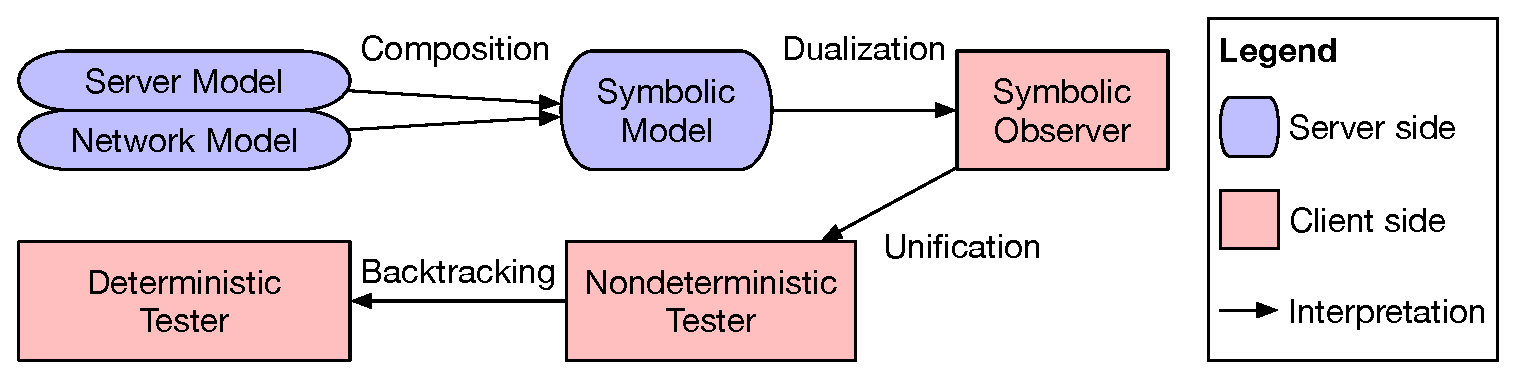
\includegraphics[width=\linewidth]{figures/framework}
  \caption{Deriving tester program from specification.}
  \label{fig:framework}
\end{figure}

\autoref{fig:framework} illustrates the derivation framework from ITrees to
testers.  \autoref{sec:itree} introduces the ITree language that encodes each
box in the framework.  \autoref{sec:internal-nondet} and
\autoref{sec:external-nondet} address internal and external nondeterminism in
the ITree context and interprets the ``server model'' into a ``nondeterministic
tester''.  \autoref{sec:backtrack} then explains how to execute the
nondterministic tester model as an interactive tester program that runs on
deterministic machines.

\section{From QAC to Interaction Trees}
\label{sec:itree}
To write specifications for protocols' rich semantics, I employed ``interaction
tree'' (ITree), a generic data structure for representing interactive programs
in the Coq programming language, introduced by \textcite{itree}.  ITree allows
specifying protocols as monadic programs that model valid implementations'
possible behavior.  The model program can be interpreted into a tester program,
to be discussed in later sections.

\subsection{Language definition}
\label{sec:itree-lang}
Consider an echo program, which keeps reading some data and writing it out
verbatim, until reaching EOF:
\begin{coq}
  CoInductive echo := c <- getchar;;
                      if c is EOF then EXIT
                      else putchar c;; echo.
\end{coq}

Here the behavior after \ilc{read} depends on the value actually read.  This
monadic computation can be desugarized into:
\begin{coq}
  CoInductive echo2 := (* equivalent to echo *)
    Bind getchar (fun c => if c is EOF then EXIT
                         else Bind (putchar c) (fun _ => echo)).
\end{coq}

\begin{figure}
\begin{coq}
  CoInductive itreeM (E: Type -> Type) (R: Type) :=
    Ret     : R   -> itreeM E R
  | Trigger : E R -> itreeM E R
  | Bind    : forall {X : Type}, itreeM E X -> (X -> itreeM E R) -> itreeM E R.
\end{coq}
\caption{Mock definition of interaction trees.}
\label{fig:mock-itree}
\end{figure}

\begin{figure}
  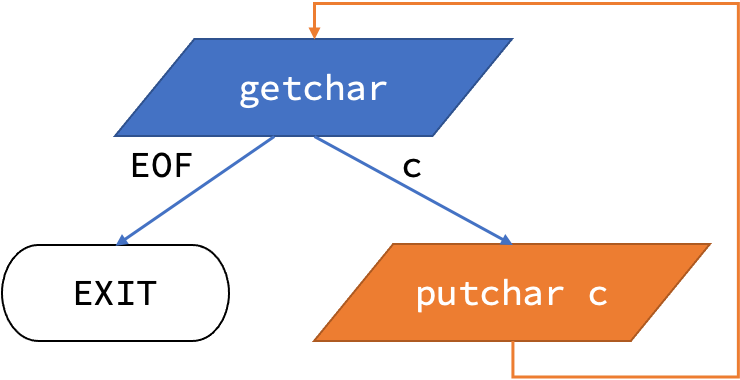
\includegraphics[width=.5\linewidth]{figures/echo-itree}
  \caption{Interaction tree for echo program}
  \label{fig:echo-itree}
\end{figure}

Such continuation-passing style can be represented as a tree of interactions.
To help readers better understand the interaction tree language, I first provide
a modified version of it that better shows its tree structure, and then explain
the actual type definition used in practice.

\paragraph{Mock interaction trees}
As shown in \autoref{fig:mock-itree}, a mock interaction tree (\ilc{itreeM}) has
two kinds of nodes, \ilc{Ret} and \ilc{Trigger}, and has edges constructed by
\ilc{Bind}:
\begin{itemize}
\item \ilc{(Ret r)} represents a pure computation that yields a value \ilc r.
  In the echo example, \ilc{EXIT} halts the program with return value zero:
\begin{coq}
  Definition EXIT {E} : itreeM E Z := Ret 0.
\end{coq}
\item \ilc{(Trigger e)} performs an impure event \ilc e and returns its result.
  Here \ilc{(e: E R)} is an event whose result is of type \ilc R.  For example,
  \ilc{getchar} has result type \ilc{char}, and \ilc{putchar}'s result type is
  \ilc{unit} (which corresponds to \inlinec{void} in C/C++, or \ilc{()} in
  Haskell).  These effective programs are constructed by triggering standard I/O
  events:
\begin{coq}
  Variant stdioE: Type -> Type := (* event type *)
    GetChar:         stdioE char
  | PutChar: char -> stdioE unit.
  
  Definition getchar : itreeM stdioE char := Trigger GetChar.
  Definition putchar (c: char) : itreeM stdioE unit
                               := Trigger (PutChar c).
\end{coq}
\item \ilc{(Bind m k)} binds the return value of \ilc m to the continuation
  function \ilc k.  It first runs program \ilc m until it returns some value of
  type \ilc X.  The return value \ilc{(x: X)} then instantiates \ilc k into the
  following computation \ilc{(k x: itreeM E R)}.  This corresponds to the
  \ilc{(;;)} syntax in \ilc{echo}:
\begin{coq}
  Notation "x <- m1;; m2" := (Bind m1 (fun x => m2)).
  Notation "m1;; m2"      := (Bind m1 (fun _ => m2)).
\end{coq}

As illustrated in \autoref{fig:echo-itree}, each possible return value \ilc x is
an edge that leads to the child it instantiates {\it i.e.} \ilc{(k x)}.  In this
way, the \ilc{Ret} and \ilc{Trigger} nodes are connected into a tree
structure.
\end{itemize}

The mock interaction tree provides an intuitive continuation-passing structure
for representing impure programs.  However, this language is not suitable for
writing specifications and deriving them into tester programs, because the test
derivation requires analyzing and transforming the specification program.

A mock interaction tree has infinitely many syntactic variants that are
semantically equivalent, due to monad laws.  For example, consider the following
programs:
\begin{coq}
  Example bind_ret  r k     := Bind (Ret r) k.
  Example bind_bind m k1 k2 := Bind (Bind m k1) k2.
\end{coq}
These programs are semantically equivalent to:
\begin{coq}
  Example bind_ret2  r k     := k r.
  Example bind_bind2 m k1 k2 := x <- m;; Bind (k1 x) k2.
\end{coq}

To make program analysis more effective, we need to redefine the tree structure
in a normal form, where each semantics corresponds to a unique syntax.  The
revised language eliminates expressions like \ilc{bind_ret} and \ilc{bind_bind}.

\paragraph{Practical interaction trees}
\footnote{For readability, the ``practical'' ITree definition here is a
  simplified version from \textcite{itree}.}
\begin{figure}
\begin{coq}
  CoInductive itree (E: Type -> Type) (R: Type) :=
    Pure   : R -> itree E R
  | Impure : forall {X : Type}, E X -> (X -> itree E R) -> itree E R.
\end{coq}
\caption{Formal definition of interaction trees}
\label{fig:itrees}
\end{figure}
The type definition of ITree restricts that only single events can be bound to a
continuation.  As shown in \autoref{fig:itrees}, I use \ilc{(Impure e k)} to
replace \ilc{(Bind (Trigger e) k)} representations in \ilc{itreeM}.  A
\ilc{Pure} computation cannot be bound to a continuation, and must be the leaf
of an ITree.

The \ilc{Ret}, \ilc{Trigger}, and \ilc{Bind} constructors introduced in
\ilc{itreeM} have equivalent representations in \ilc{itree}, so we can still
write programs in the monadic syntax:
\begin{coq}
  Definition ret {E R} : R -> itree E R := Pure.
  
  Definition trigger {E R} (e: E R) : itree E R := Impure e Pure.

  CoFixpoint bind {X E R} (m: itree E X) (f: X -> itree E R) : itree E R :=
    match m with
    | Pure   x   => f x
    | Impure e k => Impure e (fun r => bind (k r) f)
    end.

  Notation "x <- m1;; m2" := (bind m1 (fun x => m2)).
  Notation "m1;; m2"      := (bind m1 (fun _ => m2)).

  CoFixpoint translateM {E R} (m: itreeM E R) : itree E R :=
    match m with
    | Ret     r => ret r
    | Trigger e => trigger e
    | Bind m1 k => x <- translateM m1;; translateM (k x)
    end.
\end{coq}

ITrees can specify various kinds of programs like servers and testers, by
defining different event types.  For example, the QAC server in
\autoref{def:server} exhibits internal nondeterminism.  The internal choices
made by the server can be represented as \ilc{Choice} events whose result can be
any value in the space of choices:
\begin{coq}
  Variant choiceE: Type -> Type :=
    Choice: choiceE C.
\end{coq}

The server also needs to send requests and receive responses:
\begin{coq}
  Variant qaE: Type -> Type :=
    Recv: qaE Q           (* receive a request *)
  | Send: A -> qaE unit.  (* send a response   *)

  Definition qacE: Type -> Type := qaE +' choiceE.
\end{coq}

Here \ilc{qacE} is a sum type of \ilc{qaE} and \ilc{choiceE} events, meaning
that the server may send or receive messages, and may also make internal
choices.  I split the event types because they'll be handled differently when I
derive the tester later in this chapter.

Now we can represent the QAC server with step function \ilc{sstep} and initial
state \ilc{sigma}:
\begin{coq}
  CoInductive server (sstep: Q -> C -> sigma -> A * sigma) (s: sigma)
              : itree qacE void :=
    c <- trigger Choice;;
    q <- trigger Recv;;
    let (a, s') := sstep q c s in
    trigger (Send a);;
    server sstep s'.
\end{coq}

This subsection has provided a brief taste of the ITree specification language.
To construct a tester from the specification, we need to dualize the model's
behavior into the tester-side behavior, based on the theory explained in
\autoref{sec:dualization}.  To dualize specifications written in ITrees, we need
an {\em interpretation} mechanism that transforms ITrees into other programs,
which will be explained in the next subsection.

\subsection{Interpreting interaction trees}
To interpret a program \ilc p is to specify a rule that defines ``if \ilc p does
this, then do that''.  For example, shell syntax \inlinec{(p < input > output)}
executes \inlinec p but redirects its standard I/O.  Suppose \inlinec p is the
\ilc{echo} program in \autoref{sec:itree-lang}, then the redirected program
should perform file operations specified in \ilc{redirect_echo}:
\begin{coq}
  Variant fileE: Type -> Type :=      (* file operation events *)
    Fgetc: file ->         fileE char
  | Fputc: file -> char -> fileE unit.

  CoInductive redirect_echo (input output: file) : itree fileE unit :=
    c <- trigger (Fgetc input);;
    if c is EOF then ret 0
    else trigger (Fputc output c);;
         redirect_echo input output.
\end{coq}

When redirecting a program's standard I/O to files, the interpretation rule is
``whenever the program wants to read from or write to standard I/O, perform the
read/write operation on the specified file instead'':
\begin{coq}
  Definition redirect (input output: file) {R: Type} (e: stdioE R) :=
    match e in stdioE R return itree fileE R with
    | GetChar   => trigger (Fgetc input)
    | PutChar c => trigger (Fputc output c)
    end.
\end{coq}

Here the \ilc{redirect} function takes a standard I/O event and turns it into an
ITree program that performs file events.  The result program has the same return
type as the original event, so it can ``replace'' the original \ilc{stdioE}.
This is done by the \ilc{interp} function:
\begin{coq}
  CoFixpoint interp {E F R} (f: forall {T}, E T -> itree F T) (m: itree E R)
             : itree F R :=
    match m with
    | Pure   r   => Pure r
    | Impure e k => x <- f e;;
                    interp handler (k x)
    end.

  Definition redirect_echo2 (input output: file) : itree fileE unit :=
    interp (redirect input output) (translateM echo).
\end{coq}

For each impure event, the interpretor replaces it with the program defined by
the handler function \ilc f.  As a result, \ilc{redirect_echo2} constructs a
redirected echo program that is equivalent with \ilc{redirect_echo}.

To derive tester programs from ITree specifications, I'll introduce multiple
interpretation processes, with various event handlers throughout this chapter.


\section{Handling Internal Nondeterminism}
\label{sec:internal-nondet}
This section applies the idea of dualization in \autoref{chap:dualize} to the
ITree context, showing how to address internal nondeterminism by symbolic
evaluation based on ITree specifications.  It covers the derivation path from
``symbolic model'' to ``nondeterministic tester'' in \autoref{fig:framework},
using \http entity tags introduced in \autoref{sec:internal-nondeterminism} as
an example.

As discussed in \autoref{sec:encode-spec}, dualization requires refining the
representation of the server's computation {\it e.g.} encoding its branches over
symbolic conditions.  This is done by designing ITrees' event types in
\autoref{sec:symbolic-model} and specifying the server's behavior with a
symbolic model.

The server specification is derived into a tester client by {\em interpreting}
interaction trees.  To interpret is to define semantic rules that transform one
ITree program into another, and corresponds to the arrows in
\autoref{fig:framework}.  \autoref{sec:interp} explains the interpretation of
ITrees.

The interpretation from symbolic model to the nondeterministic tester model is
implemented in two phases, illustrated as ``dualization'' and ``unification''
arrows in \autoref{fig:framework}: \autoref{sec:dualize-interaction} dualizes
the server's behavior into the tester client's, resulting in a ``symbolic
observer'' that encodes symbolic evaluation as primitive events.
\autoref{sec:symbolic-eval} then instantiates the primitive events into
pure computations that unify concrete observations against their symbolic
representations.

\subsection{Symbolic server model}
\label{sec:symbolic-model}
The server specification is an ITree program that exhibits all valid behavior of
the protocol.  I combine the $\Prog$ language in \autoref{sec:prog-lang} with the
simplistic ITree example in \autoref{sec:qac-itree}.

\paragraph{Network packet type}
Instead of receiving requests and sending responses, the server receives and
sends {\em packets} that carry routing information.  This allows us to specify
the server's interaction against concurrent clients in
\autoref{sec:external-nondet}.  A packet consists of headers that indicate its
source and destination, and a payload of either a request or a response:
\begin{coq}
  Notation connection := N. (* N for natural number *)

  Record packet Q A := {
    Source      : endpoint;
    Destination : endpoint;
    Payload     : Q + A
  }.
\end{coq}
This type definition says: the \ilc{packet} type is parameterized over the \ilc
Q and \ilc A types that represent its request and response.  Its \ilc{Source}
and \ilc{Destination} fields each records an \ilc{endpoint} represented as a
natural number.  Its \ilc{Payload} type is the sum of request and response.

Here's an example trace of network packets:
\begin{coq}
  Context get: string -> request.
  Context ok : string -> response.

  Definition server_end: endpoint := 0.

  Example trace: list (packet request response) :=
    [ { Source      := 1;
        Destination := server_end;
        Payload     := inl (get "/index.html")
      }
    ; { Source      := server_end;
        Destination := 1;
        Payload     := inr (ok "<p>Hello!</p>")
      }
    ].
\end{coq}
This trace encodes a transaction between client 1 and the server (represented as
endpoint 0).  The client sends a GET request to fetch the resource in path
\ilc{"/index.html"}, and the server responds with 200 OK and content
\ilc{"<p>Hello!</p>"}.  The \ilc{inl} and \ilc{inr} are constructors for sum
types:
\begin{coq}
  Context inl: forall {X Y}, X -> X + Y.
  Context inr: forall {X Y}, Y -> X + Y.
\end{coq}

\paragraph{Symbolic representation}
To specify systems' nondeterministic behavior, the $\Prog$ language in
\autoref{sec:prog-lang} encodes data as symbolic expressions $\Sexp$, so that
the responses and branch conditions may depend on internal choices.  I do the
same for ITree specifications, by symbolizing the choice events and branch
conditions.  Take my HTTP specification~\cite{issta21} as an example.  Its
choice event has symbolic expression as result type:

\begin{coq}
  Variant comparison := Strong | Weak.

  Variant exp: Type -> Type :=
    Const    : string -> exp string
  | Var      : var    -> exp string
  | Compare  : string -> exp string -> comparison -> exp bool.

  Variant choiceE: Type -> Type :=
    Choice: choiceE (exp string).
\end{coq}

Here I instantiate the \ilc{choiceE} in \autoref{sec:itree-lang} with symbolic
return type \ilc{(exp string)}, pronounced ``expression of type string''.  In
this example, I use strings to represent entity tags (ETags) that HTTP servers
may generate, which was discussed in \autoref{sec:internal-nondeterminism}.  The
type interface can be adjusted to other protocols under test.

Symbolic expressions may be constructed as constant values, as variables, or
with operators.  Here is an example of expressions of type string:
\begin{coq}
  Context x y : var.

  Example expressions: list (exp string) :=
    [ Const   "foo"
    ; Var      x
    ; Compare "bar" (Var y) Weak
    ].
\end{coq}

The \ilc{Compare} constructor takes an expression of type string and compares it
against a constant string.  \ilc{(Compare t tx cmp)} represents the ETag
comparison between \ilc{t} and \ilc{tx}, using ``strong comparison'' or ``weak
comparison'' mechanism\footnote{\http servers may choose to generate ETags as
``strong validators'' (with uniqueness guarantee) or ``weak validators'' (for
potentially better performance).  Weak validators have prefix \iletag{W/} while
strong validators do not.  When handling compare-and-swap operations such as PUT
requests conditioned over \inlinec{If-Match} in
\autoref{sec:internal-nondeterminism}, the server should evaluate its
precondition with ``strong comparison'' that doesn't allow weak validators ({\it
e.g.} \iletag{W/"foo"}) to match any ETag including itself.  For GET requests
conditioned over \inlinec{If-None-Match}, the server may evaluate with ``weak
comparison'' where a weak validator like \iletag{W/"bar"} matches itself and
also matches strong validator \iletag{"bar"}, but doesn't match \iletag{W/"foo"}
or \iletag{"foo"}.} specified by \ilc{cmp}.  The constant ETag is provided by
the request, and the symbolic one comes from the server state.

\begin{figure}
\begin{lstlisting}[numbers=left]
  Notation sigma := (path -> resource).

  Context OK PreconditionFailed : symbolic_response.
  Context process: request -> sigma -> itree smE (symbolic_response * sigma).

  CoFixpoint server_http (state: sigma) :=
    pq <- trigger Recv;;
    let respond_with a :=
      trigger (Send { Source      := server_conn
                    ; Destination := pq.(Source)
                    ; Payload     := inr a } ) in
    let q : request    := request_of pq        in
    let v : string     := q.(Content)          in
    let k : path       := q.(TargetPath)       in
    let t : string     := if_match q           in
    let tx: exp string := (state k).(ETag)     in
    IFX (Compare t tx Strong)%\label{line:etag-ifx}%
    THEN
      if q.(Method) is Put%\label{line:etag-pure-if}%
      then
        tx' <- or (trigger Choice)%\label{line:etag-choice}%
                  (Pure (Const EmptyString));;
        let state' := state [k |-> {Content := v; ETag := tx'}] in
        respond_with OK;;
        server_http state'
      else                 (* handling other kinds of requests *)
        (a, state') <- process q state;;
        respond_with a;;
        server_http state'
    ELSE
      respond_with PreconditionFailed;;
      server_http s.%\label{line:etag-end}%
\end{lstlisting}
\caption{Server model for HTTP conditional requests}
\label{fig:if-match-server}
\end{figure}

\autoref{fig:if-match-server} shows an ITree model for If-Match requests 
(\autoref{sec:internal-nondeterminism}).  The server state \ilc{sigma} \lys{I
used \ilc{sigma} to represent the server state in QAC, so keeping this
notation.}  maps each path to its corresponding ``resource''---file content and
metadata like ETag.  The server first evaluates the request's \inlinec{If-Match}
condition by ``strong comparison'' as required by HTTP.  If the request's ETag
matches its target's, then the server updates the target's contents with the
request payload.  The target's new ETag \ilc{tx'} is permitted to be any value,
so the model represents it as \ilc{Choice} event.

Notice that the server model exhibits three kinds of branches:
\begin{enumerate}
\item The \ilc{if} branch in \autoref{line:etag-pure-if} is provided by ITree's
embedding language Coq, and takes a boolean value as condition;
\item The \ilc{IFX} branch in \autoref{line:etag-ifx} constructs an ITree that
nondeterministically branches over a condition written as a symbolic expression
of type bool:
\begin{coq}
  Variant branchE: Type -> Type :=
    Decide: exp bool -> branchE bool.

  Notation "IFX condition THEN x ELSE y" :=
    (b <- trigger (Decide condition);;
     if b then x else y).
\end{coq}
\item The \ilc{or} operator in \autoref{line:etag-choice} takes two ITrees as
possible branches and constructs an ITree that may nondeterministically take
either branch:
\begin{coq}
  Variant nondetE: Type -> Type :=
    Or: nondetE bool.

  Definition or {E R} (x y: itree E R) : itree E R :=
    b <- trigger Or;;
    if b then x else y.
\end{coq}
\end{enumerate}

These three kinds of branch conditions play different roles in the
specification, and will be handled differently during testing:
\begin{enumerate}
\item The ``pure'' \ilc{if} condition is used for deterministic branches like
  \ilc{(q.(Method) is Put)} in the example.  Here \ilc q is a ``concrete
  request''---a request that doesn't involve symbolic variables, as opposed to
  ``symbolic'' ones---generated by the client and sent to the server, so its
  method is known by the tester and needn't be symbolically evaluated.
\item The ``symbolic'' \ilc{IFX} condition here plays a similar rule as the
  $\mathsf{if}$ branches in the $\Prog$ language: Which branch to take depends
  on the server's internal choices, so the tester needs to consider both cases.
\item The \ilc{or} branch defines multiple control flows the server may take.
  In the HTTP example, the server may generate an ETag for the resource's new
  content, but is not obliged to do so.  It may choose to generate no ETags
  instead, using \ilc{(Pure (Const EmptyString))} as an alternative
  to \ilc{(trigger Choice)}.
\end{enumerate}

In addition to \ilc{IFX} branch conditions, the symbolic expressions may also
appear in the server's responses.  For example, after generating an ETag in
\autoref{line:etag-choice} of \autoref{fig:if-match-server}, the server may
receive a GET request and send the ETag to the client:
\begin{coq}
  Example ok_with_etag: symbolic_response :=
    { ResponseLine := { Version := { Major := 1; Minor := 1 }
                      ; Code    := 200
                      ; Phrase  := OK
                      }
    ; ResponseFields :=
      [ { Name := "Content-Length"; Value := Const "13" }
      ; { Name := "ETag"          ; Value := Var    x   }
      ]
    ; ResponseBody := "<p>Hello!</p>"
    }.
\end{coq}
Suppose the server generated the ETag as expression \ilc{(Var x)}, then we can
use the expression to construct the symbolic response in the specification,
rather than determining its concrete value.  The mechanism of producing
expressions for ETags is explained in \autoref{sec:dualize-interaction}.

Now we can define the specification's event type \ilc{smE}.  The symbolic server
model receives concrete requests and sends symbolic responses, so its event is
defined as:
\begin{coq}
  Definition symbolic_packet := packet request symbolic_response.

  Definition qaE := ioE symbolic_packet symbolic_packet.

  Notation smE := (qaE +' nondetE +' choiceE +' branchE).
\end{coq}
The ``Symbolic Model'' in \autoref{fig:framework} is an ITree constructed by
applying the \ilc{server_http} function to an initial state:
\begin{coq}
  Definition sm_http: itree smE void :=
    server_http init_state.
\end{coq}

The rest of this section will explain the interpretations from this symbolic
model.

\subsection{Dualizing symbolic model}
\label{sec:dualize-interaction}
This subsection takes the symbolic model composed in
\autoref{sec:symbolic-model} and dualizes its interactions, which corresponds
to the ``Dualization'' arrow in \autoref{fig:framework}.  It applies the idea of
derivation rules (\ref{rule:write})--(\ref{rule:return}) for $\Prog$
(\autoref{sec:dualize-prog}) to models written as ITrees.

This interpretation phase produces a symbolic observer that models the tester's
observation and validation behavior.  The observer sends a request when the
server wants to receive one, and receives a response when the server wants to
send one.  It also creates constraints over the server's internal choices based
on its observations.

\autoref{fig:symbolic-observer} shows the dualization algorithm.  It interprets
the symbolic model's events with the \ilc{observe} handler, whose types are
explained as follows:

\begin{figure}
\begin{lstlisting}[numbers=left]
Notation oE := (observeE +' nondetE +' choiceE +' constraintE).

Definition observe {R} (e: smE R) : itree oE R :=
  match e with
  | Recv      => trigger FromObserver%\label{line:observe-absorb}%
  | Send px   => p <- trigger ToObserver;;%\label{line:observe-emit}%
                 trigger (Guard px p)
  | Decide bx => or (trigger (Unify bx true);;  ret true)%\label{line:observe-branch}%
                    (trigger (Unify bx false);; ret false)
  | Or        => trigger Or%\label{line:observe-or}%
  | Choice    => trigger Choice%\label{line:observe-choice}%
  end.

Definition observer_http: itree oE void :=
  interp observe sm_http.
\end{lstlisting}
\caption{Dualizing symbolic model into symbolic observer.}
\label{fig:symbolic-observer}
\end{figure}

The tester observes a trace of concrete packets, so observer's interactions
return concrete requests and responses, as opposed to the symbolic model whose
responses are symbolic.
\begin{coq}
  Definition concrete_packet := packet request concrete_response.

  Variant observeE : Type -> Type :=
    FromObserver   : observeE concrete_packet
  | ToObserver     : observeE concrete_packet.
\end{coq}

Notice that the observer's send and receive events both return the packet sent
or received, unlike the server model whose \ilc{Send} event takes the sent
packet as argument.  This is because the tester needs to generate the request
packet to send, and the event's result value represents that generated and sent
packet.

As discussed in \autoref{sec:dualize-prog}, when the server sends a symbolic
response or branches over a symbolic condition, the tester needs to create
symbolic constraints accordingly.  The observer introduces ``constraint events''
to represent the creation of constraints primitively.
\begin{coq}
  Variant constraintE : Type -> Type :=
    Guard : packet -> concrete_packet -> constraintE unit
  | Unify : exp bool -> bool -> constraintE unit.
\end{coq}

Here \ilc{(Guard px p)} creates a constraint that the symbolic packet \ilc{px}
emitted by the specification matches the concrete packet \ilc p observed during
runtime.  \ilc{(Unify bx b)} creates a constraint that unifies the symbolic
branch condition \ilc{bx} with boolean value \ilc b.  These constraints will be
solved in \autoref{sec:symbolic-eval}.

The dualization algorithm in \autoref{fig:symbolic-observer} does the follows:
\begin{enumerate}
  \item When the symbolic model absorbs a packet in
    \autoref{line:observe-absorb}, the observer generates a request packet;
  \item When the symbolic model emits a symbolic packet \ilc{px} in
    \autoref{line:observe-emit}, the observer receives a concrete packet \ilc p,
    and adds a constraint that restricts the symbolic and concrete packets to
    match each other.
  \item When the symbolic model branches on a symbolic condition \ilc{bx} in
    \autoref{line:observe-branch}, the tester accepts the observation if it can
    be explained by any branch.  This is done by constructing the observer as a
    nondeterministic program that has both branches, using the \ilc{or}
    combinator.  For each branch, the observer adds a constraint that the
    symbolic condition matches the chosen branch.
  \item Nondeterministic branches in \autoref{line:observe-or} are preserved in
    this interpretation phase, and will be resolved in \autoref{sec:backtrack}.
  \item Internal choices in \autoref{line:observe-choice} are addressed by the
    next phase in \autoref{sec:symbolic-eval}, along with the constraints
    created in this phase.
\end{enumerate}

The result of dualization is a symbolic observer that models tester behaviors
like sending requests and receiving responses.  The symbolic observer is a
nondeterministic program with primitives events like making choices and adding
constraints over the choices.

For example, dualizing \autoref{line:etag-ifx}--\ref{line:etag-end} in
\autoref{fig:if-match-server} results in an observer program as shown in
\autoref{fig:observer-example}.  The next subsection interprets the observer's
primitive \ilc{Guard} and \ilc{Unify} events into pure computations of symbolic
evaluation.

\begin{figure}
\begin{coq}
  Example observer_body: itree oE void :=
    let guard_response a :=
      p <- trigger ToObserver;;
      trigger (Guard { Source      := server_conn
                     ; Destination := pq.(Source)
                     ; Payload     := inr a } ) in
    let bx: exp bool := Compare t tx Strong in
    or (
        trigger (Unify (Compare bx true));;
        if q.(Method) is Put
        then
          tx' <- or (trigger Choice)
                    (Pure (Const EmptyString));;
          let state' := state [k |-> {Content := v; ETag := tx'}] in
          guard_response OK;;
          interp observe (server_http state')
        else
          (a, state') <- interp observe (process q state);;
          guard_response a;;
          interp observe (server_http state')
       )
       (
        trigger (Unify (Compare bx false));;
        guard_response PreconditionFailed;;
        interp observe (server_http s)
       ).
\end{coq}
\caption{Symbolic observer example.}
\label{fig:observer-example}
\end{figure}


\subsection{Symbolic evaluation}
\label{sec:symbolic-eval}
This subsection takes the symbolic observer produced in
\autoref{sec:dualize-interaction} and solves the constraints it has created.
The constraints unify symbolic packets and branch conditions against the
concrete observations.  The tester should accept the SUT if the constraints are
satisfiable.

\begin{figure}
\begin{lstlisting}[numbers=left]
Notation ntE := (observeE +' nondetE +' exceptE).

Definition V: Type := list var * list (constraintE unit).
  
Definition unify {R} (e: oE R) (v: V) : itree ntE (V * R) :=
  let (xs, cs) := v in
  match e with
  | Choice => let x: var := fresh v in%\label{line:unify-choice}%
              ret (x::xs, cs, Var x)
  | (constraint: unifyE) => let cs' := constraint::cs in%\label{line:unify-constraint}%
                            if solvable cs'
                            then ret (xs, cs', tt)
                            else Trigger (Throw ("Conflict: " ++ print cs'))
  | Or             => b <- trigger Or;; ret (v, b)%\label{line:unify-or}%
  | (oe: observeE) => r <- trigger oe;; ret (v, r)%\label{line:unify-observe}%
  end.

Definition nondet_tester_http: itree ntE void :=
  (_, vd) <- interp_state unify observer_http initV;;
  match vd in void with end.
\end{lstlisting}
\caption{Resolving symbolic constraints.}
\label{fig:nondet-tester}
\end{figure}

As shown in \autoref{fig:nondet-tester}, the unification algorithm evaluates the
primitive symbolic events into a stateful checker program, which reflects the
$\Prog$-based validator in \autoref{sec:dualize-prog}.  The interpreter
maintains a validation state \ilc V which stores the symbolic variables and the
constraints over them.  The derivation rules are as follows:
\begin{enumerate}
  \item When the server makes an internal choice in \autoref{line:unify-choice},
    the tester creates a fresh variable and adds it to the validation state.
  \item When the observer creates a constraint in
    \autoref{line:unify-constraint}, the tester adds the constraint to the
    validation state, and solves the new set of constraints.  If the constraints
    become unsatisfiable, then the tester \ilc{Throw}s an exception that
    indicates the current execution branch cannot accept the observations:
\begin{coq}
  Variable exceptE: Type -> Type :=
    Throw: forall {X}, string -> exceptE X.
\end{coq}
  \item The observer is a nondeterministic program with multiple execution
    paths, constructed by \ilc{Or} events in \autoref{line:unify-or}.  The
    tester accepts the observation if any of the branches does not throw an
    exception.  These branches will be handled in the next section, along with
    the observer's send/receive interactions in \autoref{line:unify-observe}.
\end{enumerate}

Notice that the \ilc{unify} function interprets a symbolic observer's event
\ilc{(oE R)} into a function of type \ilc{(V -> itree tE (V * R))}, which is
also called a state monad transformer.  It takes a pre-validation state \ilc{(v:
V)} and computes an ITree that yields the observer event's corresponding result
\ilc{(r: R)} along with a post-validation state \ilc{(v': V)}.  This stateful
interpretation process is implemented by a variant of \ilc{interp} called
\ilc{interp_state}:
\begin{coq}
  CoFixpoint interp_state {E F V R}
                          (handler: forall {X}, E X -> V -> itree F (V * X))
                          (m: itree E R) (v: V)
             : itree F (V * R) :=
    match m with
    | Pure   r   => ret (v, r)
    | Impure e k => '(v', r) <- handler e v;;
                    interp_state handler (k r) v'
    end.
\end{coq}

So far I have interpreted the symbolic model into a tester model that observes
incoming and outgoing packets, nondeterministically branches, and in some cases
throws exceptions.  Next I'll explain how to extend the symbolic model to
address external nondeterminism.


\section{Handling External Nondeterminism}
\label{sec:external-nondet}
As introduced in \autoref{sec:intro-external-nondet}, the environment might
affect the transmission of messages, so called external nondeterminism.  The
tester should take the environment into account when validating its
observations.

This section explains how to address external nondeterminism by specifying the
environment, using the networked server example.  It corresponds to the
``Composition'' arrow in \autoref{fig:framework}.  \autoref{sec:net-tcp} defines
a model for concurrent TCP connections.  \autoref{sec:net-compose} then composes
the network model with the server specification, yielding a tester-side
specification that defines the space of valid observations.

\subsection{Modelling the network}
\label{sec:net-tcp}
When testing servers over the network, request and response packets may be
delayed.  As a result, messages from one end might arrive at the
other end in a different order from that they were sent.

The space of network reorderings can be modelled by a {\em network model}, a
conceptual program for the ``network wire''.  The wire can be viewed as a
buffer, which absorbs packets\footnote{In this section, ``packet'' is a
shorthand for the ``symbolic packet'' defined on
Page~\pageref{def:symbolic-packet}.} and later emits them:
\begin{coq}
  Notation packet := symbolic_packet.

  Definition netE: Type -> Type :=
    ioE packet packet.

  Notation Absorb := Recv.
  Notation Emit   := Send.
\end{coq}

For example, the network model for concurrent TCP connections is defined in
\autoref{fig:tcp-model}.  The model captures TCP's feature of maintaining the
order within each connection, but packets in different connections might be
reordered arbitrarily.  When the wire chooses a packet to send, the candidate
must be the oldest in its connection.

\begin{figure}
\begin{coq}
(* filter the oldest packet in each connection *)
Context oldest_in_each_conn : list packet -> list packet.

Fixpoint pick_one (l: list packet) : itree nondetE (option packet) :=
  if l is p::l'
  then or (Ret (Some p)) (pick_one l')
  else ret None.

CoFixpoint tcp (buffer: list packet) : itree (netE +' nondetE) void :=
  let absorb := pkt <- trigger Absorb;;
                tcp (buffer ++ [pkt])      in
  let emit p := trigger (Emit p);;
                tcp (remove pkt buffer)    in
  let pkts   := oldest_in_each_conn buffer in
  opkt <- pick_one pkts;;
  if opkt is Some pkt
  then emit pkt
  else absorb.
\end{coq}
\caption[Network model for concurrent TCP connections]{Network model for
  concurrent TCP connections.  The model is an infinite program iterating over a
  \ilc{buffer} of all packets en route.  In each iteration, the model either
  \ilc{absorb}s or \ilc{emit}s some packet, depending on the current
  \ilc{buffer} state and the choice made in \ilc{pick_one}.  Any absorbed packet
  is appended to the end of buffer.  When emitting a packet, the model may
  choose a connection and send the oldest packet in it.}
\label{fig:tcp-model}
\end{figure}

Notice the \ilc{pick_one} function, which might return (i) \ilc{Some p} or (ii)
\ilc{None}.  The network model then (i) emits packet \ilc p or (ii) absorbs a
packet into \ilc{buffer}.

\begin{itemize}
\item When the given list \ilc{pkts} is empty, \ilc{pick_one} always returns
  \ilc{None}, because the wire has no packet in the \ilc{buffer}, and must
  absorb some packet before emitting anything.
\item Given a non-empty linked list \ilc{(p::l')}, with \ilc p as head and
  \ilc{l'} as tail, \ilc{pick_one} might return \ilc{(Some p)}, meaning the wire
  can emit that packet; or it might return \ilc{None}, meaning the wire can
  still absorb packets into the buffer.
\end{itemize}

Such network model reflects the TCP environment, where messages are never lost
but might be indefinitely delayed.  In the next subsection, I'll demonstrate how
to compose the server and network models into a client-side observation model.

\subsection{Network composition}
\label{sec:net-compose}

The network connects the server on one end to the clients on other ends.  When
one end sends some message, the network model absorbs it and later emits it to
the destination.

To {\em compose} a server model with a network model is to pair the server's
\ilc{Send} and \ilc{Recv} events with the network's \ilc{Absorb} and \ilc{Emit}
events.  Since the network model is nondeterministic, it might not be ready at
some given moment to absorb packets sent by the server.  The network might also
emit a packet before the server is ready to receive it.

\begin{figure}
  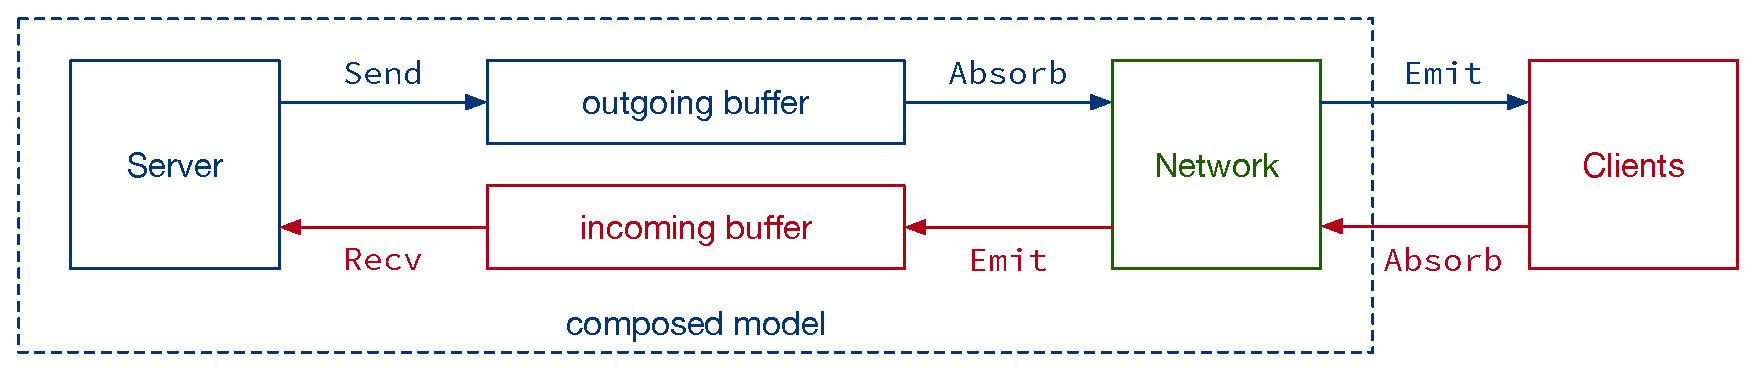
\includegraphics[width=\textwidth]{figures/net-compose}
  \caption{Network composition architecture}
  \label{fig:net-compose}
\end{figure}

To handle the asynchronicity among the server and network events, I insert
message buffers between them.  As shown in \autoref{fig:net-compose}, the {\em
  incoming buffer} stores the packets emitted by the network but not yet
consumed by the server's \ilc{Recv} events, and the {\em outgoing buffer} stores
the packets sent by the server but not yet absorbed by the network.

\begin{figure}
\begin{lstlisting}[numbers=left]
CoFixpoint compose {E} (srv: itree smE void)          (* server  model *)
           (net  : itree (netE +' nondetE) void)      (* network model *)
           (bi bo: list packet)       (* incoming and outgoing buffers *)
           : itree (netE +' nondetE +' E) void :=
  let step_net :=%\label{line:step-net-def}%
    match net with
    | Impure Absorb knet =>
      match bo with
      | pkt::bo' => compose srv (knet pkt) bi bo'%\label{line:net-absorb}%
      | []       => pkt <- trigger Absorb;;%\label{line:client-send}%
                    compose srv (knet pkt) bi bo
      end
    | Impure (Emit pkt) knet =>%\label{line:net-emit}%
      if toServer pkt
      then compose srv (knet tt) (bi++[pkt]) bo%\label{line:srv-incoming}%
      else trigger (Emit pkt);;%\label{line:net-send}%
           compose srv (knet tt) bi bo
    | Impure Or knet => b <- trigger Or;;
                      compose srv (knet b) bi bo
    | Pure vd => match vd in void with end
    end
  in
  match srv with
  | Impure Recv ksrv =>%\label{line:srv-recv}%
    match bi with
    | pkt::bi' => compose (ksrv pkt) net bi' bo%\label{line:srv-consume}%
    | [] => step_net%\label{line:step-net}%
    end
  | Impure (Send pkt) ksrv =>%\label{line:srv-send}%
    compose (ksrv tt) net bi (bo++[pkt])
  | Impure e ksrv =>        (* other events performed by the server *)
    r <- trigger e;; compose (ksrv r) net bi bo
  | Pure vd => match vd in void with end
  end.
\end{lstlisting}
\caption[Network composition algorithm]{Network composition algorithm.  When the
  server wants to send a packet in \autoref{line:srv-send}, the packet is
  appended to the outgoing buffer until absorbed by the network
  in \autoref{line:net-absorb}, and eventually emitted to the client
  in \autoref{line:net-send}.  Conversely, a packet sent by the client is
  absorbed by the network in \autoref{line:client-send}, emitted to the server's
  incoming buffer in \autoref{line:srv-incoming}, until the server consumes it
  in \autoref{line:srv-consume}.}
\label{fig:net-compose-code}
\end{figure}

The server and the clients are the opposite ends of the network.  Each packet
has routing fields that indicate its source and destination.  When the network
emits a packet, we need to determine whether the packet is emitted to the
server's incoming buffer or to the clients, by inspecting its destination:
\begin{coq}
  Definition toServer (p: packet) : bool :=
    if p.(Destination) is server_conn then true else false.
\end{coq}

Now we can define the composition algorithm formally, as shown in
\autoref{fig:net-compose-code}.  The function takes the symbolic server model
in \autoref{sec:symbolic-model} and the network model in \autoref{sec:net-tcp},
and yields a symbolic model of the server's behavior observable from across the
network.

The composition function analyzes the server and the network's behavior:
\begin{enumerate}
\item When the server wants to send a packet in \autoref{line:srv-send}, the
packet is appended to the outgoing buffer.
\item When the network wants to absorb a packet in \autoref{line:net-absorb},
it first checks whether the server has sent some packet to its outgoing buffer.
If yes, then the network absorbs the oldest packet in the buffer.  Otherwise, it
absorbs from the clients.
\item After absorbing some packets, when the network wants to emit a packet in
\autoref{line:net-emit}, the packet is either emitted to the client or appended
to the server's incoming buffer, based on its destination.
\item When the server wants to receive a packet in \autoref{line:srv-recv},
it first checks whether the network has emitted some packet to the incoming
buffer.  If yes, then the server takes the oldest packet in the buffer.
Otherwise, it waits for the network model to emit one.
\end{enumerate}

Notice that this algorithm schedules the server at a higher priority than the
network model.  The composed model only steps into the network model when the
server is starved in \autoref{line:step-net}, by calling the \ilc{step_net}
process defined in \autoref{line:step-net-def}.  This design is to avoid
divergence of the derived tester program, which I'll further explain in
\autoref{sec:backtrack}.

So far I've shown how to specify systems that exhibit external nondeterminism.
By specifying the environment and composing it with the implementation-side
specification, we can describe the space of valid observations.  The rest of
this chapter will show how to derive tester programs from the observer-side
specification.


\section{Executing the Tester Model}
\label{sec:backtrack}
This section takes the nondetermistic tester model derived in
\autoref{sec:symbolic-eval} and transforms it into an interactive program.
\autoref{sec:backtracking} handles the nondeterministic branches via backtrack
execution, and produces a deterministic tester model.  \autoref{sec:itree-io}
then interprets the deterministic tester into IO program that interacts with the
SUT.

\subsection{Backtrack execution}
\label{sec:backtracking}
This subsection explains how to run the nondeterministic tester on a
deterministic machine.  It reflects the derivation rules (\ref{rule:unsat}) and
(\ref{rule:reject}) for $\Prog$ in \autoref{sec:dualize-prog}, and constructs
the ``Backtracking'' arrow in \autoref{fig:framework}.

The deterministic tester implements a client that sends and receives concrete
packets:
\begin{coq}
  Variant clientE: Type -> Type :=
    ClientSend: concrete_packet -> clientE unit
  | ClientRecv: clientE (option concrete_packet).
\end{coq}

Notice that the \ilc{ClientRecv} event might return \ilc{(Some pkt)}, indicating
that the SUT has sent a packet \ilc{pkt} to the tester; or it might
return \ilc{None}, when the SUT is silent or its sent packet hasn't arrived at
the tester side.  This allows the tester to perform non-blocking interactions,
instead of waiting for the SUT which might cause starvation.

\begin{figure}
\begin{lstlisting}[style=customcoq,numbers=left,escapechar=\%]
Notation tE := (clientE +' genE +' exceptE).

CoFixpoint backtrack (current:      itree ntE void)
                     (others: list (itree ntE void))
           : itree tE void :=
  match current with
  | Impure e k =>
    match e with
    | (|Or|)          => b <- trigger GenBool;;%\label{line:backtrack-or}%
                         backtrack (k b) (k (negb b)::others)
    | (||Throw msg)   => match others with%\label{line:backtrack-throw}%
                         | other::ot' => backtrack other ot'
                         | []         => trigger (Throw msg)
                         end
    | (FromObserver|) => q <- GenPacket;;
                         trigger (ClientSend q);;%\label{line:backtrack-send}%
                         let others' := expect FromObserver q others in
                         backtrack (k q) others'
    | (ToObserver|)   =>
      oa <- trigger ClientRecv;;%\label{line:backtrack-recv}%
      match oa with
      | Some oa => let others' := expect ToObserver a others in
                   backtrack (k a) others'
      | None    =>%\label{line:backtrack-silent}%
        match others with
        | other::ot' => backtrack other (ot'++[current]) (* postpone *)%\label{line:backtrack-postpone}%
        | []         => backtrack m     []               (* retry    *)
        end
      end
    end
  | Pure vd => match vd in void with end
  end.

Definition tester_http: itree tE void :=
  backtrack nondet_tester_http [].
\end{lstlisting}
\caption{Backtrack execution of nondeterministic tester.}
\label{fig:backtrack}
\end{figure}

\autoref{fig:backtrack} shows the backtracking algorithm.  It interacts with the
SUT and checks whether the observations can be explained by the nondeterministic
tester model.  That is, checking whether the tester has an execution path that
matches its interactions.  This is done by maintaining a list of all possible
branches in the tester, and checking if any of them accepts the observation.

The tester exhibits two kinds of randomness: (1) When sending a request packet
to the SUT, it generates the packet randomly with \ilc{GenPacket}; (2) When the
nondeterministic tester model branches, the deterministic tester randomly picks
one branch to evaluate, using \ilc{GenBool}:
\begin{coq}
  Variant genE: Type -> Type :=
    GenPacket: genE concrete_packet
  | GenBool  : genE bool.
\end{coq}

\begin{figure}
\begin{lstlisting}[style=customcoq,numbers=left,escapechar=\%]
CoFixpoint match_observe {R} (e: observeE R) (r: R)
                             (m: itree ntE (V * void))
           : itree ntE (V * void) :=
  match m with
  | Impure (oe|) k =>
    match oe, e with
    | FromObserver, FromObserver%\label{line:match-from}%
    | ToObserver  , ToObserver => k r%\label{line:match-to}%
    | _, _ => trigger (Throw ("Expect " ++ print oe%\label{line:match-throw}%
                           ++ " but observed " ++ print e))
    end
  | Impure (|e0|) k | Impure (||e0) k =>
    r0 <- trigger e0;;
    match_observe e r (k r0)
  | Pure (_, vd) => match vd in void with end
  end.

Definition expect {R} (e: observeE R) (r: R)
  : list (itree ntE (V * void)) -> list (itree ntE (V * void))
  := map (match_observe e r).
\end{lstlisting}
\caption{Matching tester model against existing observation.}
\label{fig:match-observe}
\end{figure}

The execution rule is defined as follows:
\begin{enumerate}
\item When the tester nondeterministically branches
  in \autoref{line:backtrack-or}, randomly pick a branch \ilc{(k b)} to
  evaluate, and push the other branch \ilc{(k (negb b))} to the list of other
  possible cases.

\item When the \ilc{current} tester throws an exception in
  \autoref{line:backtrack-throw}, it indicates that the current execution path
  rejects the observations.  The tester should try to explain its observations
  with other branches of the tester model.  If the \ilc{others} list is empty,
  it indicates that the observation is beyond the specification's producible
  behavior, so the tester should reject the SUT.

\item When the tester wants to observe a packet {\em from} itself, it generates
  a packet and sends it to the SUT in \autoref{line:backtrack-send}.

  Notice that if the current branch is rejected and the tester backtracks to
  other branches, the sent packet cannot be recalled from the environment.
  Therefore, all other branches should be matched against this send event as
  well.  This is done by the \ilc{expect} function.
  
  As shown in \autoref{fig:match-observe}, \ilc{(expect e r l)} matches every
  tester in list \ilc l against the observation \ilc e that has return
  value \ilc r.  For each element $\texttt m\in\texttt l$, if \ilc m's first
  observer event \ilc{oe} matches the observation \ilc e
  (\autoref{line:match-from} and \autoref{line:match-to}),
  then \ilc{match_observe} instantiates the tester's continuation function \ilc
  k with the observed result \ilc r.  Otherwise, the tester throws an exception
  in \autoref{line:match-throw}, indicating that this branch cannot explain the
  observation because they performed different events.
  \label{rule:backtrack-send}

\item When the current tester wants to observe a packet {\em to} itself, it
  triggers the \ilc{ClientRecv} event in \autoref{line:backtrack-recv}.  If a
  packet has indeed arrived, then it instantiates the current branch as well as
  other possible branches, in the same way as discussed
  in Rule~(\ref{rule:backtrack-send}).

  If the tester hasn't received a packet from the SUT
  (\autoref{line:backtrack-silent}), it doesn't reject the SUT, because the
  expected packet might be delayed in the environment.  If there are \ilc{other}
  branches to evaluate (\autoref{line:backtrack-postpone}), then the tester
  postpones the \ilc{current} branch by appending it to the back of the queue.
  Otherwise, if the current branch is the only one that hasn't rejected, then
  the tester retries the receive interaction.

  Notice that if the SUT keeps silent, then the tester will starve but won't
  reject, because (i) such silence is indistinguishable from the SUT sending a
  packet but delayed by the environment, and (ii) the SUT hasn't {\em exhibited}
  any violations against the specification.  The starvation issue is addressed
  in \autoref{sec:itree-io}.
\end{enumerate}

The backtracking algorithm also explains the network composition design
in \autoref{fig:net-compose-code}, where the server model is scheduled at a
higher priority than the network model: Suppose the SUT has produced some
invalid output, then every branch of the tester should reject its observation by
throwing an exception.  However, the network model is always ready to absorb
packets.  Evaluating the network model lazily prevents the composed symbolic
model from having infinitely many absorbing branches.  This allows the derived
tester to converge to rejection upon violation.

Now we have derived the specification into a deterministic tester model in
ITree.  The tester's events reflect actual computations of a client program.  In
the next subsection, I'll translate the ITree model into a binary executable
that runs on silicon and metal.

\subsection{From ITree model to IO program}
\label{sec:itree-io}
The deterministic tester model derived in \autoref{fig:backtrack} is an ITree
program that never returns (its result type \ilc{void} has no elements).  It
represents a client program that keeps interacting with the SUT until it reveals
a violation and throws an exception.

In practice, if the tester hasn't found any violation after performing a certain
amount of interactions, then it accepts the SUT.  This is done by executing the
ITree until reaching a certain depth.

\begin{figure}
\begin{lstlisting}[style=customcoq,numbers=left,escapechar=\%]
Fixpoint execute (fuel: nat) (m: itree tE void) : IO bool :=
  match fuel with
  | O       => ret true               (* accept if out of fuel *)%\label{line:execute-accept}%
  | S fuel' =>
    match m with
    | Impure e k =>
      match e with
      | (||Throw _)     => ret false  (* reject upon exception *)%\label{line:execute-reject}%
      | (ClientSend q|) => client_send q;;
                           execute fuel' (k tt)
      | (ClientRecv|)   => oa <- client_recv;;
                           execute fuel' (k oa)
      | (|GenPacket|)   => pkt <- gen_packet;;%\label{line:execute-gen}%
                           execute fuel' (k pkt)
      | (|GenBool|)     => b <- ORandom.bool;;
                           execute fuel' (k b)
      end
    | Pure vd => match vd in void with end
    end
  end.

Definition test_http: IO bool :=
  execute bigNumber tester_http.
\end{lstlisting}
\caption{Interpreting ITree tester to IO monad.}
\label{fig:execute}
\end{figure}

As shown in \autoref{fig:execute}, the \ilc{execute} function takes an
argument \ilc{fuel} that indicates the remaining depth to explore in the ITree.
If the execution ran out of fuel (\autoref{line:execute-accept}), then the test
accepts; If the tester model throws an exception
(\autoref{line:execute-reject}), then the test rejects.  Otherwise, it
translates the ITree's primitive events into IO computations in Coq \lys{Cite
Li-yao's SimpleIO library}, which are eventually extracted into OCaml programs
that can be compiled into executables that can communicate with the SUT over the
operating system's network stack.

This concludes my validation methodology.  In this chapter, I have shown how to
test real-world systems that exhibit internal and external nondeterminism.  I
applied the dualization theory in \autoref{chap:theory} to address internal
nondetermism, and handled external nondeterminism by specifying the
environment's space of uncertainty.  The specification is derived into an
executable tester program, by multiple phases of interpretations.  The
derivation framework is built on the ITree specification language, but the
method is applicable to other languages that allow destructing and analyzing the
model programs.

So far I have answered ``how to tell compliant implementations from violating
ones''.  The next chapter will answer ``how to generate and shrink test input
that reveal violations effectively'', and unveil the techniques behind
\ilc{gen_packet} in \autoref{line:execute-gen} of \autoref{fig:execute}.

